\documentclass[aspectratio=169,10pt]{beamer}

%% ─────────────────────────────────────────────
%%  THEME & COLORS
%% ─────────────────────────────────────────────
\usetheme{Madrid}
\usecolortheme{seahorse}

\definecolor{RLBlue}{RGB}{0,64,128}
\definecolor{RLRed}{RGB}{180,0,0}
\definecolor{RLGreen}{RGB}{0,120,60}
\definecolor{RLOrange}{RGB}{200,90,0}
\definecolor{RLGray}{RGB}{80,80,80}
\definecolor{SafeGreen}{RGB}{0,140,70}
\definecolor{RobustPurple}{RGB}{100,0,150}
\definecolor{ExplainTeal}{RGB}{0,120,130}
\definecolor{SlideGray}{RGB}{240,242,245}

\setbeamercolor{palette primary}{bg=RLBlue,fg=white}
\setbeamercolor{palette secondary}{bg=RLBlue!80,fg=white}
\setbeamercolor{palette tertiary}{bg=RLBlue!60,fg=white}
\setbeamercolor{palette quaternary}{bg=RLBlue,fg=white}
\setbeamercolor{structure}{fg=RLBlue}
\setbeamercolor{block title}{bg=RLBlue,fg=white}
\setbeamercolor{block title example}{bg=SafeGreen,fg=white}
\setbeamercolor{block title alerted}{bg=RLRed,fg=white}
\setbeamercolor{frametitle}{bg=RLBlue,fg=white}

%% ─────────────────────────────────────────────
%%  PACKAGES
%% ─────────────────────────────────────────────
\usepackage[T1]{fontenc}
\usepackage[utf8]{inputenc}
\usepackage{lmodern}
\usepackage{amsmath,amssymb,amsfonts,amsthm}
\usefonttheme[onlymath]{serif}
\usepackage{graphicx,booktabs,array,multicol}
\usepackage{tikz,pgfplots}
\usepackage{listings}
\usepackage{hyperref}
\usepackage{fontawesome5}
\usepackage{tcolorbox}
\pgfplotsset{compat=1.18}
\usetikzlibrary{shapes.geometric,arrows.meta,positioning,fit,backgrounds,calc}

\tcbuselibrary{skins,breakable}

%% ─────────────────────────────────────────────
%%  CUSTOM BOXES
%% ─────────────────────────────────────────────
\newtcolorbox{paperbox}[1]{
  colback=RLBlue!6, colframe=RLBlue,
  title={\protect\faIcon{file-alt}\ #1},
  fonttitle=\bfseries\small, fontupper=\small,
  boxrule=0.8pt, arc=3pt
}
\newtcolorbox{industrybox}[1]{
  colback=SafeGreen!8, colframe=SafeGreen,
  title={\protect\faIndustry\ #1},
  fonttitle=\bfseries\small, fontupper=\small,
  boxrule=0.8pt, arc=3pt
}
\newtcolorbox{warnbox}[1]{
  colback=RLRed!6, colframe=RLRed,
  title={\protect\faExclamationTriangle\ #1},
  fonttitle=\bfseries\small, fontupper=\small,
  boxrule=0.8pt, arc=3pt
}
\newtcolorbox{mathbox}{
  colback=RLBlue!4, colframe=RLBlue!50,
  boxrule=0.6pt, arc=3pt
}

%% ─────────────────────────────────────────────
%%  CODE LISTING STYLE
%% ─────────────────────────────────────────────
\lstset{
  basicstyle=\ttfamily\scriptsize,
  keywordstyle=\bfseries\color{RLBlue},
  commentstyle=\itshape\color{RLGray},
  stringstyle=\color{SafeGreen},
  numbers=left, numberstyle=\tiny\color{RLGray},
  frame=single, rulecolor=\color{RLBlue!40},
  backgroundcolor=\color{SlideGray},
  xleftmargin=10pt, breaklines=true
}

%% ─────────────────────────────────────────────
%%  FOOTER CUSTOMISATION
%% ─────────────────────────────────────────────
\setbeamertemplate{footline}{%
  \leavevmode%
  \hbox{%
    \begin{beamercolorbox}[wd=.34\paperwidth,ht=2.4ex,dp=1ex,center]{palette primary}%
      \usebeamerfont{author in head/foot}%
      \faLinkedin\ linkedin.com/in/abdullahzahid655
    \end{beamercolorbox}%
    \begin{beamercolorbox}[wd=.34\paperwidth,ht=2.4ex,dp=1ex,center]{palette secondary}%
      \usebeamerfont{title in head/foot}%
      \faGithub\ github.com/abdullahzahid655
    \end{beamercolorbox}%
    \begin{beamercolorbox}[wd=.32\paperwidth,ht=2.4ex,dp=1ex,right]{palette tertiary}%
      \usebeamerfont{date in head/foot}%
      \insertshortsubtitle\ \quad \insertframenumber/\inserttotalframenumber\hspace*{2ex}
    \end{beamercolorbox}%
  }%
}
\setbeamertemplate{navigation symbols}{}

%% ─────────────────────────────────────────────
%%  METADATA
%% ─────────────────────────────────────────────
\author[Abdullah Zahid]{%
  \textbf{Abdullah Zahid} \\[2pt]
  \small\faLinkedin\ \href{https://linkedin.com/in/abdullahzahid655}{linkedin.com/in/abdullahzahid655}
  \quad \faGithub\ \href{https://github.com/abdullahzahid655}{github.com/abdullahzahid655}
}
\title[RL Roadmap — Phase 6]{Reinforcement Learning Roadmap}
\subtitle{Phase 6: Safety, Robustness \& Explainability}
\vspace{3pt}
\institute[RL Learning Series]{Deep Reinforcement Learning Journey \\ \textit{Professional Learning Series}}
\date{\today}

%% ─────────────────────────────────────────────
%%  SECTION DIVIDER
%% ─────────────────────────────────────────────
\AtBeginSection[]{
  \begin{frame}[plain]
    \begin{tikzpicture}[remember picture, overlay]
      \fill[RLBlue] (current page.south west) rectangle (current page.north east);
      \node[white, font=\Huge\bfseries, align=center, text width=0.8\paperwidth] 
            at (current page.center) {\insertsection};
      \node[white!70, font=\large] at ([yshift=-1.8cm]current page.center)
            {Phase 6: Safety, Robustness \& Explainability};
    \end{tikzpicture}
  \end{frame}
}

%% ═══════════════════════════════════════════════════════
\begin{document}
%% ═══════════════════════════════════════════════════════

%% ─── TITLE PAGE ────────────────────────────────────────
\begin{frame}[plain]
  \begin{tikzpicture}[remember picture, overlay]
    \fill[RLBlue!95] (current page.south west) rectangle (current page.north east);
    %% decorative stripe
    \fill[RLOrange] ([yshift=-0.8pt]current page.north west) rectangle
                    ([yshift=-6pt]current page.north east);
  \end{tikzpicture}
  \vspace{0.8cm}
  \begin{center}
    {\color{white}\Large\textbf{Reinforcement Learning Roadmap}}\\[4pt]
    {\color{RLOrange}\rule{0.55\textwidth}{1pt}}\\[6pt]
    {\color{white}\LARGE\bfseries Phase 6: Safety, Robustness \& Explainability}\\[10pt]
    {\color{white!80}\normalsize
      Making RL Agents Trustworthy, Resilient, and Transparent for the Real World}\\[18pt]
    {\color{white}\small
      \faLinkedin\ \href{https://linkedin.com/in/abdullahzahid655}{\color{RLOrange}linkedin.com/in/abdullahzahid655}
      \quad\textbf{|}\quad
      \faGithub\ \href{https://github.com/abdullahzahid655}{\color{RLOrange}github.com/abdullahzahid655}}\\[6pt]
    {\color{white!60}\small\today}
  \end{center}
\end{frame}

%% ─── TABLE OF CONTENTS ─────────────────────────────────
\begin{frame}{Roadmap — Phase 6 at a Glance}
  \begin{columns}
    \column{0.55\textwidth}
      \tableofcontents
    \column{0.42\textwidth}
      \begin{tcolorbox}[colback=RLBlue!8,colframe=RLBlue,title=\textbf{Why Phase 6?},
                        fonttitle=\small\bfseries,fontupper=\small]
        Phases 1–5 taught us \emph{how} to train RL agents.\\[4pt]
        Phase 6 answers the harder question:\\[2pt]
        \textbf{Can we trust them in the real world?}\\[6pt]
        \begin{itemize}\setlength\itemsep{2pt}
          \item {\color{SafeGreen}\faShield*} Safety constraints
          \item {\color{RobustPurple}\faBolt} Robustness to attacks
          \item {\color{ExplainTeal}\faEye} Explainable decisions
        \end{itemize}
      \end{tcolorbox}
  \end{columns}
\end{frame}

%% ─── PHASE RECAP ───────────────────────────────────────
\begin{frame}{Our Journey So Far}
  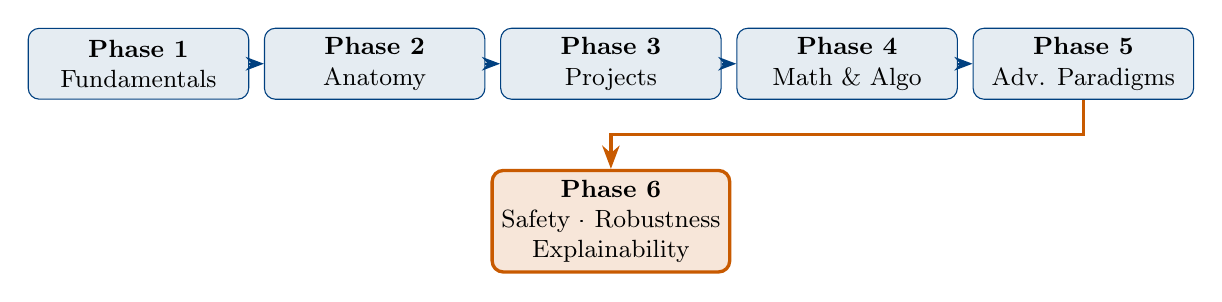
\begin{tikzpicture}[every node/.style={font=\small},
    phase/.style={draw=RLBlue,fill=RLBlue!10,rounded corners=4pt,
                  minimum width=2.8cm,minimum height=0.9cm,align=center},
    cur/.style={draw=RLOrange,fill=RLOrange!15,rounded corners=4pt,
                minimum width=2.8cm,minimum height=0.9cm,align=center,
                very thick},
    arr/.style={-Stealth,RLBlue,thick}]
    \node[phase] (p1) at (0,0) {\textbf{Phase 1}\\Fundamentals};
    \node[phase] (p2) at (3,0) {\textbf{Phase 2}\\Anatomy};
    \node[phase] (p3) at (6,0) {\textbf{Phase 3}\\Projects};
    \node[phase] (p4) at (9,0) {\textbf{Phase 4}\\Math \& Algo};
    \node[phase] (p5) at (12,0) {\textbf{Phase 5}\\Adv. Paradigms};
    \node[cur]   (p6) at (6,-2) {\textbf{Phase 6}\\Safety · Robustness\\Explainability};
    \draw[arr] (p1)--(p2); \draw[arr] (p2)--(p3);
    \draw[arr] (p3)--(p4); \draw[arr] (p4)--(p5);
    \draw[arr,RLOrange,very thick] (p5) -- ++(0,-0.9) -| (p6);
  \end{tikzpicture}

  \begin{center}
    {\color{RLOrange}\textbf{Phase 6}} bridges advanced paradigms with \textbf{real-world deployment requirements}
  \end{center}
\end{frame}

%% ══════════════════════════════════════════════════
\section{Safe Reinforcement Learning}
%% ══════════════════════════════════════════════════

\begin{frame}[t]{What Is Safe RL?}
  \vspace{-20pt}
  \begin{columns}[T]
    \column{0.52\textwidth}
      \begin{block}{Core Formulation: CMDP}
        \textbf{Constrained Markov Decision Process} extends the standard MDP
        by adding cost signals and budget constraints:
        \begin{mathbox}
          \begin{align*}
            \max_{\pi}\quad &\mathbb{E}_{\pi}\!\left[\sum_{t=0}^{\infty}\gamma^t r_t\right]\\
            \text{s.t.}\quad
            &\mathbb{E}_{\pi}\!\left[\sum_{t=0}^{\infty}\gamma^t c_t\right] \le b
          \end{align*}
        \end{mathbox}
        where $c_t$ is a \textbf{cost signal} and $b$ is the \textbf{safety budget}.
      \end{block}
      
      \vspace{-6pt}
      
      \begin{alertblock}{The Core Tension}
        \centering
        \textbf{Higher reward} $\longleftrightarrow$ \textbf{Lower safety}\\
        SafeRL learns the Pareto frontier between them.
      \end{alertblock}
    \column{0.45\textwidth}
      \begin{exampleblock}{Real-World Motivation}
        \begin{itemize}\setlength\itemsep{3pt}
          \item \textbf{Autonomous Driving}: minimize travel time \emph{while} ensuring low accident probability [Wachi et al., 2024]
          \item \textbf{Power Grids}: optimise electricity production \emph{while} maintaining reliability standards
          \item \textbf{Robotics}: reach target \emph{without} collisions
          \item \textbf{Healthcare}: maximise patient outcome \emph{within} dosage limits
        \end{itemize}
      \end{exampleblock}
  \end{columns}
\end{frame}

\begin{frame}{Safe RL Algorithm Families}
  \begin{columns}[T]
    \column{0.32\textwidth}
      \begin{tcolorbox}[colback=SafeGreen!8,colframe=SafeGreen,
                        title=\textbf{Lagrangian Methods},fonttitle=\small\bfseries]
        \small
        Convert constrained problem to unconstrained via dual variable $\lambda$:
        \begin{equation*}
          \mathcal{L}(\pi,\lambda)=J^r-\lambda(J^c-b)
        \end{equation*}
        \textbf{Examples:}
        \begin{itemize}\setlength\itemsep{1pt}
          \item PPO-Lagrangian
          \item TRPO-Lagrangian
          \item PID Lagrangian
        \end{itemize}
        \textbf{Pro:} Simple drop-in\\
        \textbf{Con:} Oscillation risk
      \end{tcolorbox}
    \column{0.32\textwidth}
      \begin{tcolorbox}[colback=RLBlue!8,colframe=RLBlue,
                        title=\textbf{Trust-Region Methods},fonttitle=\small\bfseries]
        \small
        Constrain both reward and cost updates within a safe trust region.
        \begin{equation*}\pi_{k+1}=\arg\max_\pi J^r \text{ s.t. cost}\le b\end{equation*}
        \textbf{Examples:}
        \begin{itemize}\setlength\itemsep{1pt}
          \item CPO (Achiam et al., 2017)
          \item PCPO
          \item SB-TRPO (2024)
        \end{itemize}
        \textbf{Pro:} Monotonic safety\\
        \textbf{Con:} Computationally heavy
      \end{tcolorbox}
    \column{0.32\textwidth}
      \begin{tcolorbox}[colback=RLOrange!8,colframe=RLOrange,
                        title=\textbf{Model-Based Methods},fonttitle=\small\bfseries]
        \small
        Predict cost using a world model, plan safely before execution.
        \textbf{Examples:}
        \begin{itemize}\setlength\itemsep{1pt}
          \item SafeDreamer (ICLR 2024)
          \item MOPO + cost model
          \item CBF-based control
        \end{itemize}
        \textbf{Pro:} Near-zero violations\\
        \textbf{Con:} Model errors propagate
      \end{tcolorbox}
  \end{columns}
\end{frame}

\begin{frame}{Constrained Policy Optimization (CPO)}
  \begin{columns}[T]
    \column{0.52\textwidth}
    \vspace{-15pt}
      \begin{block}{CPO — Achiam et al., ICML 2017}
        Updates policy within a trust region \emph{and} respects cost constraints simultaneously:
        \begin{mathbox}
          \begin{align*}
            \pi_{k+1} &= \arg\max_{\pi}\quad J^r(\pi) \\
            \text{s.t.}\quad
              &J^c(\pi) \le b \\
              &D_{KL}(\pi\|\pi_k) \le \delta
          \end{align*}
        \end{mathbox}
        Uses first-order Taylor approximation + line-search to solve efficiently.
      \end{block}
      
      \begin{paperbox}{Key Paper}
        Achiam, J. et al. (2017). \textit{Constrained Policy Optimization}. ICML 2017.
        Wachi, A. et al. (2024). \textit{A Survey of Constraint Formulations in Safe RL.} arXiv:2402.02025
      \end{paperbox}
    \column{0.45\textwidth}
    \vspace{-15pt}
      \begin{exampleblock}{SafeDreamer: World-Model Safety}
        Integrates Lagrangian methods into world model planning (Dreamer framework):
        \begin{enumerate}\setlength\itemsep{2pt}\small
          \item World model trained from replay buffer
          \item Lagrangian planner optimises in latent space
          \item Achieves \textbf{near-zero cost} on Safety-Gymnasium
        \end{enumerate}
      \end{exampleblock}
      \vspace{4pt}
      \begin{paperbox}{Key Paper}
        Huang, W. et al. (2024). \textit{SafeDreamer: Safe RL with World Models.} ICLR 2024. arXiv:2307.07176
      \end{paperbox}
  \end{columns}
\end{frame}

\begin{frame}{Safe RL: Industry Deployments}
  \begin{columns}[T]
    \column{0.48\textwidth}
    \vspace{-11pt}
      \begin{industrybox}{Autonomous Driving — Waymo / Tesla}
        \small
        \begin{itemize}\setlength\itemsep{2pt}
          \item Constrained RL for lane-keeping and intersection navigation
          \item Reward: minimize travel time
\item Constraints: collision probability $< 10^{-6}$ per mile
          \item Uses shielding layers as hard safety overrides
        \end{itemize}
      \end{industrybox}
      \vspace{1pt}
      \begin{industrybox}{Robotic Arm — Industrial Automation}
        \small
        \begin{itemize}\setlength\itemsep{1pt}
          \item Adjei et al. (2024): CMDP for arm manipulation avoiding human operators
          \item Lagrange multiplier $\lambda$ adapts dynamically to danger proximity
          \item Published in \textit{Robotics, MDPI 2024}
        \end{itemize}
      \end{industrybox}
    \column{0.48\textwidth}
    \vspace{-11pt}
      \begin{industrybox}{Power Grid — Energy Management}
        \small
        \begin{itemize}\setlength\itemsep{2pt}
          \item Optimise energy dispatch (reward) while satisfying reliability constraints (cost)
          \item Risk-sensitive CVaR constraints guard against brownouts
          \item Used in smart-grid pilot programs
        \end{itemize}
      \end{industrybox}
      \vspace{6pt}
      \begin{industrybox}{Multi-Agent Safe RL — Drone Swarms}
        \small
        \begin{itemize}\setlength\itemsep{2pt}
          \item Scal-MAPPO-L (NeurIPS 2024): scalable safe MARL for drone coordination
          \item Decentralised execution with local constraint satisfaction
          \item Handles 50+ drones simultaneously
        \end{itemize}
      \end{industrybox}
  \end{columns}
\end{frame}

\begin{frame}{Control Barrier Functions (CBF) for Hard Safety}
  \begin{columns}[T]
    \column{0.50\textwidth}
      \begin{block}{CBF — Hard Safety Guarantee}
        A function $h(s)$ is a CBF if the set $\mathcal{C}=\{s:h(s)\ge 0\}$ is \textbf{forward-invariant}:
        \begin{mathbox}
          \begin{equation*}
            \dot{h}(s,a) + \alpha(h(s)) \ge 0 \quad \forall s\in\mathcal{C}
          \end{equation*}
        \end{mathbox}
        Combined with RL: the RL policy proposes actions, CBF \emph{projects} them to the safe set.
      \end{block}
      \begin{itemize}\setlength\itemsep{2pt}\small
        \item No constraint violations \emph{by construction}
        \item Works in continuous action spaces
        \item Used in safety-critical robotics
      \end{itemize}
    \column{0.46\textwidth}
      \begin{tcolorbox}[colback=RLBlue!5,colframe=RLBlue,title=\textbf{Safe RL Taxonomy},
                        fonttitle=\small\bfseries]
        \small
        \begin{tabular}{@{}ll@{}}
          \toprule
          \textbf{Approach} & \textbf{Guarantee} \\
          \midrule
          Lagrangian & Soft, expectation \\
          CPO / Trust-Region & Soft, monotonic \\
          CBF Shielding & Hard, formal \\
          CMDP offline & Soft, offline data \\
          SafeDreamer & Near-zero, model \\
          \bottomrule
        \end{tabular}
      \end{tcolorbox}
      \vspace{4pt}
      \begin{paperbox}{Survey}
        Garcia \& Fernández (2015). \textit{Comprehensive Survey on Safe RL}. JMLR 16(1).\\[2pt]
        Gu et al. (2024). \textit{A Survey of Safe RL}. IEEE TPAMI 2024.
      \end{paperbox}
  \end{columns}
\end{frame}

%% ══════════════════════════════════════════════════
\section{Robust Reinforcement Learning}
%% ══════════════════════════════════════════════════

\begin{frame}{Why Robustness Matters}
  \begin{columns}[T]
    \column{0.50\textwidth}
    \vspace{-11pt}
      \begin{warnbox}{The Brittleness Problem}
        DRL agents achieve superhuman performance in controlled environments, but:
        \begin{itemize}\setlength\itemsep{2pt}\small
          \item Small observation perturbations \emph{collapse} performance
          \item A self-driving agent with GPS noise drifts off-road
          \item Sim-to-real gap invalidates trained policies
          \item Adversarial attackers can deliberately exploit vulnerabilities
        \end{itemize}
      \end{warnbox}
      \vspace{-10pt}
      \begin{block}{State-Adversarial MDP (SA-MDP)}
        \begin{mathbox}
          \vspace{-15pt}
          \begingroup
          \footnotesize
          \begin{equation*}
            \Omega^{\xi} = (S, A, T, R, \mathcal{X}, O^{\xi})
          \end{equation*}
          \endgroup
        \end{mathbox}
        Adversary modifies observations: $O^{\xi}(x_t|s_t)$
        Agent must perform well under \textbf{worst-case} perturbations.
      \end{block}
    \column{0.46\textwidth}
    \vspace{-11pt}
      \begin{exampleblock}{Types of Adversarial Attacks}
        \begin{enumerate}\setlength\itemsep{3pt}\small
          \item \textbf{Observation Attacks}: perturb agent's state input\\
            {\color{RLGray}$\rightarrow$ FGSM, PGD variants}
          \item \textbf{Action Attacks}: corrupt agent's actuator output\\
            {\color{RLGray}$\rightarrow$ NR-MDP framework}
          \item \textbf{Reward Attacks}: manipulate reward signal\\
            {\color{RLGray}$\rightarrow$ Reward poisoning}
          \item \textbf{Dynamics Attacks}: change environment physics\\
            {\color{RLGray}$\rightarrow$ Domain-shift attacks}
          \item \textbf{Adversarial Policy}: co-agent manipulates behaviour\\
            {\color{RLGray}$\rightarrow$ Gleave et al., ICLR 2020}
        \end{enumerate}
      \end{exampleblock}
  \end{columns}
\end{frame}

\begin{frame}{Adversarial Training Framework}
  \begin{columns}[T]
    \column{0.52\textwidth}
    \vspace{-17pt}
      \begin{block}{Minimax Robust Objective}
        \begin{mathbox}
          \vspace{-10pt}
          \max_{\pi}\;\min_{\xi\in\Xi}\;\mathbb{E}_{\pi,\xi}\!\left[\sum_{t}\gamma^t r_t\right]
        \end{mathbox}
        Train protagonist $\pi$ against strongest possible adversary $\xi$.\par\vspace{4pt}
        \textbf{ATLA (Alternating Training of Learned Adversary):}
        \begin{enumerate}\small\setlength\itemsep{2pt}
          \item Train optimal adversary $\xi^*$ against current $\pi$
          \item Train $\pi$ against current $\xi^*$
          \item Alternate until convergence
        \end{enumerate}
      \end{block}
      \begin{paperbox}{Key Papers}
        Zhang et al. (2020). \textit{Robust DRL against Adversarial Perturbations.} NeurIPS 2020.\\
        Schott et al. (2024). \textit{Robust DRL Through Adversarial Attacks and Training.} arXiv:2403.00420
      \end{paperbox}
    \column{0.44\textwidth}
    \vspace{-15pt}
      \begin{tcolorbox}[colback=RobustPurple!6,colframe=RobustPurple,
                        title=\textbf{Robustness Techniques},fonttitle=\small\bfseries]
        \small
        \textbf{Training-Time:}
        \begin{itemize}\setlength\itemsep{1pt}
          \item Domain Randomisation
          \item Adversarial Observation Training
          \item Noise Augmentation (NA-PPO)
          \item RADIAL-RL: adversarial loss regularisation
        \end{itemize}
        \vspace{4pt}
        \textbf{Test-Time:}
        \begin{itemize}\setlength\itemsep{1pt}
          \item Certified robustness (CROP)
          \item Ensemble voting
          \item Input preprocessing / detection
        \end{itemize}
        \vspace{4pt}
        \textbf{Evaluation:}
        \begin{itemize}\setlength\itemsep{1pt}
          \item GWC (Greedy Worst-Case Reward)
          \item Attack-agnostic benchmarks
        \end{itemize}
      \end{tcolorbox}
    \end{columns}
\end{frame}

\begin{frame}{Domain Randomisation: Sim-to-Real}
  \begin{columns}[T]
    \column{0.50\textwidth}
    \vspace{-12pt}
      \begin{block}{Core Idea}
        Randomise environment parameters during training so the policy learns to generalise:
        \begin{itemize}\setlength\itemsep{3pt}\small
          \item Friction, mass, gravity coefficients
          \item Sensor noise levels
          \item Lighting \& textures (for vision)
          \item Actuator delays and latency
        \end{itemize}
        Policy sees distribution $p(\xi)$ of environments $\Rightarrow$ robust to real-world variations.
      \end{block}
      \begin{paperbox}{Notable Work}
        OpenAI (2019): \textit{Dexterous In-Hand Manipulation} — robotic hand solving Rubik's cube via massive domain randomisation. \\ 
        Chen et al. (2024). \textit{Adversarial Domain Randomization for Dual-UAV Cooperation.}
      \end{paperbox}
    \column{0.46\textwidth}
      \begin{industrybox}{Sim-to-Real Examples}
        \textbf{Boston Dynamics Atlas:}
        \begin{itemize}\setlength\itemsep{1pt}\small
          \item Trained in simulation with randomised terrain
          \item Zero-shot transfer to physical robot
        \end{itemize}
        \textbf{Industrial Assembly Robots:}
        \begin{itemize}\setlength\itemsep{1pt}\small
          \item Part orientation variance
          \item Tool wear randomisation
          \item Successfully deployed in BMW factories
        \end{itemize}
        \textbf{UAV Drone Swarms:}
        \begin{itemize}\setlength\itemsep{1pt}\small
          \item Wind disturbance randomisation
          \item Communication latency variance
          \item NeurIPS 2024: Scal-MAPPO-L
        \end{itemize}
      \end{industrybox}
    \end{columns}
\end{frame}

\begin{frame}{RADIAL-RL: Certified Adversarial Robustness}
  \begin{columns}[T]
    \column{0.50\textwidth}
      \begin{block}{RADIAL-RL Framework}
        Trains agents with \textbf{adversarial loss} as a regulariser:
        \begin{mathbox}
          \begin{equation*}
            \mathcal{L}_{total} = \mathcal{L}_{RL} + \lambda_{adv}\cdot\mathcal{L}_{adv}
          \end{equation*}
        \end{mathbox}
        where $\mathcal{L}_{adv}$ is the worst-case loss over the $l_p$-ball perturbation set.\\[4pt]
        Compatible with: DQN, A3C, PPO\\
        Tested on: Atari, MuJoCo, ProcGen
      \end{block}
      \begin{paperbox}{Paper}
        Oikarinen et al. (2021). \textit{Robust DRL Through Adversarial Loss.} NeurIPS 2021. \url{https://github.com/tuomaso/radial_rl_v2}
      \end{paperbox}
    \column{0.46\textwidth}
      \begin{tcolorbox}[colback=RobustPurple!8,colframe=RobustPurple,
                        title=\textbf{Benchmark Results (Pong)},fonttitle=\small\bfseries]
        \small
        \begin{tabular}{@{}lcc@{}}
          \toprule
          \textbf{Method} & \textbf{Clean} & \textbf{Under Attack} \\
          \midrule
          Vanilla DQN & 21 & \textcolor{RLRed}{$-$21} \\
          SA-DQN & 21 & \textcolor{SafeGreen}{21} \\
          RADIAL-DQN & 21 & \textcolor{SafeGreen}{20} \\
          \bottomrule
        \end{tabular}
        \vspace{4pt}\\
        SA-DQN / RADIAL-DQN maintain full performance under PGD attacks that \emph{completely destroy} vanilla DQN.
      \end{tcolorbox}
    \end{columns}
\end{frame}

%% ══════════════════════════════════════════════════
\section{\texorpdfstring{Explainable Reinforcement\\ Learning (XRL)}{Explainable Reinforcement Learning (XRL)}}
%% ══════════════════════════════════════════════════

\begin{frame}{The Black-Box Problem in RL}
  \begin{columns}[T]
    \column{0.50\textwidth}
    \vspace{-11pt}
      \begin{warnbox}{Why Is RL Hard to Explain?}
        \begin{itemize}\setlength\itemsep{3pt}\small
          \item Policies are \textbf{deep neural networks} — millions of parameters
          \item Decisions depend on \textbf{sequences of states} (temporal credit)
          \item Emergent strategies arise from complex reward shaping
          \item Standard XAI (LIME, SHAP) was designed for supervised learning
        \end{itemize}
      \end{warnbox}
      \vspace{-1pt}
      \begin{block}{Definition: XRL}
        \textit{``Explainable RL (XRL) is an emerging subfield that aims to elucidate the decision-making process of RL agents, enabling practitioners to understand \textbf{what} agents will do and \textbf{why}.''} [Milani et al., ACM 2023]
      \end{block}
    \column{0.46\textwidth}
      \begin{exampleblock}{Stakeholder Questions XRL Answers}
        \begin{enumerate}\setlength\itemsep{3pt}\small
          \item \textbf{Why} did the agent take action $a$ in state $s$?
          \item \textbf{What} features matter most to the policy?
          \item \textbf{When} does the agent fail or behave unexpectedly?
          \item \textbf{How} will the policy behave on unseen states?
          \item \textbf{What} subgoals is the agent pursuing?
        \end{enumerate}
      \end{exampleblock}
      \vspace{4pt}
      \begin{paperbox}{Surveys}
        Bekkemoen, Y. (2024). \textit{XRL: Systematic Literature Review and Taxonomy.} Machine Learning 113.\\[2pt]
        Milani et al. (2023). \textit{XRL: A Survey and Comparative Review.} ACM Comput. Surv.
      \end{paperbox}
  \end{columns}
\end{frame}

\begin{frame}{XRL Taxonomy}
  \begin{center}
  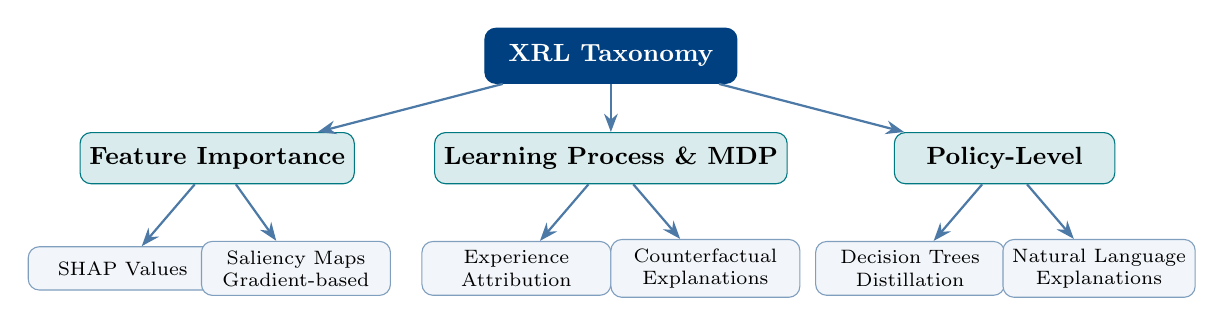
\begin{tikzpicture}[
    root/.style={draw=RLBlue,fill=RLBlue,text=white,rounded corners,
                 font=\small\bfseries,minimum width=3.2cm,minimum height=0.7cm},
    l1/.style={draw=ExplainTeal,fill=ExplainTeal!15,rounded corners,
               font=\small\bfseries,minimum width=2.8cm,minimum height=0.65cm},
    l2/.style={draw=RLBlue!50,fill=RLBlue!5,rounded corners,
               font=\scriptsize,minimum width=2.4cm,minimum height=0.55cm,align=center},
    arr/.style={-Stealth,RLBlue!70,thick}]
    \node[root] (root) {XRL Taxonomy};
    \node[l1] (fi)  at (-5,-1.3)  {Feature Importance};
    \node[l1] (lp)  at (0,-1.3)   {Learning Process \& MDP};
    \node[l1] (pl)  at (5,-1.3)   {Policy-Level};
    \draw[arr] (root)--(fi); \draw[arr] (root)--(lp); \draw[arr] (root)--(pl);

    \node[l2] (fi1) at (-6.2,-2.7) {SHAP Values};
    \node[l2] (fi2) at (-4.0,-2.7) {Saliency Maps\\Gradient-based};
    \draw[arr] (fi)--(fi1); \draw[arr] (fi)--(fi2);

    \node[l2] (lp1) at (-1.2,-2.7) {Experience\\Attribution};
    \node[l2] (lp2) at (1.2,-2.7)  {Counterfactual\\Explanations};
    \draw[arr] (lp)--(lp1); \draw[arr] (lp)--(lp2);

    \node[l2] (pl1) at (3.8,-2.7)  {Decision Trees\\Distillation};
    \node[l2] (pl2) at (6.2,-2.7)  {Natural Language\\Explanations};
    \draw[arr] (pl)--(pl1); \draw[arr] (pl)--(pl2);
  \end{tikzpicture}
  \end{center}
  \vspace{2pt}
  \centering
  {\small Based on Milani et al. (2023) ACM Computing Surveys taxonomy.}
\end{frame}

\begin{frame}{SHAP for RL: Shapley Values}
  \begin{columns}[T]
    \column{0.52\textwidth}
    \vspace{-11pt}
      \begin{block}{Shapley Value Attribution}
        Assign credit to each feature $i$ for the Q-value:
        \begin{mathbox}
          \phi_i = \sum_{S\subseteq F\setminus\{i\}}
          \frac{|S|!(|F|-|S|-1)!}{|F|!}
          \bigl[v(S\cup\{i\})-v(S)\bigr]
        \end{mathbox}
        $\phi_i > 0$: feature \emph{increased} action value\\
        $\phi_i < 0$: feature \emph{decreased} action value
      \end{block}
      \vspace{4pt}
      \begin{paperbox}{Application: XRL Governance}
        Pakina et al. (2024). \textit{AI Governance via XRL for Adaptive Cyber Deception in Zero-Trust Networks.} JISEM 2024.\\[2pt]
        SHAP raised decision transparency from \textbf{0\%} to \textbf{94\%}.
      \end{paperbox}
    \column{0.44\textwidth}
      \begin{tcolorbox}[colback=ExplainTeal!8,colframe=ExplainTeal,
                        title=\textbf{SHAP in RL Pipeline},fonttitle=\small\bfseries]
        \small
        \begin{enumerate}\setlength\itemsep{3pt}
          \item Train DQN / PPO agent normally
          \item Wrap Q-network with SHAP explainer
          \item For each state $s$, compute $\phi_i$ for all features
          \item Visualise as bar plot or heatmap
          \item Audit: do top features make sense?
        \end{enumerate}
        \vspace{4pt}
        \textbf{Libraries:}\\
        \texttt{shap}, \texttt{captum} (PyTorch)
      \end{tcolorbox}
    \end{columns}
\end{frame}

\begin{frame}{Policy Distillation: Interpretable Surrogates}
  \begin{columns}[T]
    \column{0.50\textwidth}
    \vspace{-5pt}
      \begin{block}{Core Idea}
        Distil a trained DNN policy into a simpler, interpretable model:
        \begin{enumerate}\setlength\itemsep{2pt}\small
          \item Train a high-performing DNN policy $\pi_{DNN}$
          \item Generate a large dataset of $(s, \pi_{DNN}(s))$ pairs
          \item Fit an interpretable model: decision tree, linear model, rule list
          \item Use surrogate for deployment \& auditing
        \end{enumerate}
      \end{block}
      \begin{paperbox}{Research}
        Dhebar et al. (2024). \textit{Toward Interpretable-AI Policies Using Evolutionary Nonlinear Decision Trees.} IEEE Trans. Cybern.\\[2pt]
        Beechey et al. (2023). \textit{Explaining RL with Shapley Values.} ICML 2023.
      \end{paperbox}
    \column{0.46\textwidth}
      \begin{tcolorbox}[colback=ExplainTeal!8,colframe=ExplainTeal,
                        title=\textbf{Interpretable Surrogates},fonttitle=\small\bfseries]
        \small
        \begin{tabular}{@{}lll@{}}
          \toprule
          \textbf{Surrogate} & \textbf{Fidelity} & \textbf{Interpretability} \\
          \midrule
          Linear Model & Medium & Very high \\
          Decision Tree & Medium & High \\
          Rule List & Medium & Very high \\
          Shallow NN & High & Low \\
          Prototype & High & Medium \\
          \bottomrule
        \end{tabular}
      \end{tcolorbox}
      \vspace{4pt}
      \begin{exampleblock}{XRL-SHAP-Cache}
        Hu et al. (2024, Springer). Combined DRL + SHAP for \textbf{intelligent edge service caching} in 5G CDNs — decisions fully auditable by network engineers.
      \end{exampleblock}
  \end{columns}
\end{frame}

\begin{frame}{Counterfactual Explanations in XRL}
  \begin{columns}[T]
    \column{0.50\textwidth}
    \vspace{-11pt}
      \begin{block}{What Are Counterfactuals?}
        \textit{``What \textbf{minimal change} to state $s$ would cause the agent to take a \textbf{different action}?''}
        \begin{mathbox}
          s^{CF} = \arg\min_{s'}\|s'-s\|
          \text{ s.t. } \pi(s^{CF}) \ne \pi(s)
        \end{mathbox}
        Counterfactuals provide \textbf{actionable} explanations — they tell users what \emph{would have been different.}
      \end{block}
      \vspace{4pt}
      \begin{paperbox}{Research}
        Amitai et al. (2024). \textit{Explaining RL Agents through Counterfactual Action Outcomes.} AAAI 2024.\\[2pt]
        GANterfactual-RL: visual counterfactuals for Atari agents (2023).
      \end{paperbox}
    \column{0.46\textwidth}
      \begin{exampleblock}{Healthcare XRL Example}
        \textbf{Clinical Decision Support:}
        \begin{itemize}\setlength\itemsep{2pt}\small
          \item RL optimises treatment dosing
          \item Doctor asks: \textit{Why did you recommend dose X?}
          \item SHAP shows: \textit{creatinine level was the deciding feature}
          \item Counterfactual: \textit{if creatinine $< 1.2$, dose would be Y}
        \end{itemize}
      \end{exampleblock}
      \vspace{4pt}
      \begin{paperbox}{Medical XRL}
        Ali et al. (2024). \textit{XRL for Alzheimer's Disease Progression Prediction: SHAP-based Approach.} AAAI XAI4DRL Workshop 2024.
      \end{paperbox}
  \end{columns}
\end{frame}

%% ══════════════════════════════════════════════════
\section{Connecting Phase 5 + Phase 6}
%% ══════════════════════════════════════════════════

\begin{frame}{Phase 5 $\times$ Phase 6: Synergies}
  \begin{columns}[T]
    \column{0.50\textwidth}
      \begin{block}{Safe MARL}
        Multi-agent systems with safety constraints:
        \begin{itemize}\setlength\itemsep{2pt}\small
          \item NeurIPS 2024: \textbf{Scal-MAPPO-L} — scalable safe MARL for drone swarms
          \item MACPO: Multi-Agent Constrained Policy Optimisation
          \item Challenge: individual vs shared safety constraints
        \end{itemize}
      \end{block}
      \vspace{4pt}
      \begin{block}{Robust Meta-Learning}
        Meta-RL + robustness to task distribution shifts:
        \begin{itemize}\setlength\itemsep{2pt}\small
          \item Adapt quickly to new tasks without losing safety
          \item Distributionally robust MAML
          \item Offline safe meta-RL
        \end{itemize}
      \end{block}
    \column{0.46\textwidth}
      \begin{block}{Explainable HRL}
        Hierarchical policies are naturally more interpretable:
        \begin{itemize}\setlength\itemsep{2pt}\small
          \item High-level goal is human-readable (\textit{``go to kitchen''})
          \item Low-level actions can be audited per subgoal
          \item Counterfactuals at task-decomposition level
        \end{itemize}
      \end{block}
      \vspace{-1pt}
      \begin{block}{Safe Offline RL}
        FISOR (ICLR 2024): combines offline RL + hard safety constraints:
        \begin{itemize}\setlength\itemsep{2pt}\small
          \item Feasibility-guided decoupled learning
          \item Hamilton-Jacobi reachability for safe region detection
          \item Best safety on DSRL benchmark
        \end{itemize}
      \end{block}
  \end{columns}
\end{frame}

%% ══════════════════════════════════════════════════
\section{Practical Resources}
%% ══════════════════════════════════════════════════

\begin{frame}{Key Research Papers — Phase 6}
  \begin{columns}[T]
    \column{0.48\textwidth}
      \begin{tcolorbox}[colback=SafeGreen!6,colframe=SafeGreen,
                        title=\protect\faShield*\ \textbf{Safe RL},fonttitle=\small\bfseries]
        \scriptsize
        \begin{itemize}\setlength\itemsep{2pt}
          \item Achiam et al. (2017). \textit{CPO.} ICML.
          \item Garcia \& Fernández (2015). \textit{Survey on Safe RL.} JMLR.
          \item Huang et al. (2024). \textit{SafeDreamer.} ICLR. arXiv:2307.07176
          \item Wachi et al. (2024). \textit{Survey on Constraint Formulations.} arXiv:2402.02025
          \item Liu et al. (2024). \textit{FISOR: Feasibility-guided Safe Offline RL.} ICLR.
          \item NeurIPS 2024. \textit{Scal-MAPPO-L.} Safe Multi-Agent RL.
        \end{itemize}
      \end{tcolorbox}
    \column{0.48\textwidth}
      \begin{tcolorbox}[colback=RobustPurple!6,colframe=RobustPurple,
                        title=\protect\faBolt\ \textbf{Robust RL},fonttitle=\small\bfseries]
        \scriptsize
        \begin{itemize}\setlength\itemsep{2pt}
          \item Zhang et al. (2020). \textit{SA-DQN.} NeurIPS Spotlight.
          \item Oikarinen et al. (2021). \textit{RADIAL-RL.} NeurIPS.
          \item Schott et al. (2024). \textit{Survey: Adversarial Attacks \& Training.} arXiv:2403.00420
          \item Liu et al. (2024). \textit{Safe offline RL + distributional robustness.} NeurIPS.
        \end{itemize}
      \end{tcolorbox}
  \end{columns}
  \vspace{6pt}
  \begin{tcolorbox}[colback=ExplainTeal!6,colframe=ExplainTeal,
                    title=\protect\faEye\ \textbf{Explainable RL},fonttitle=\small\bfseries]
    \scriptsize
    Bekkemoen (2024). \textit{XRL Systematic Literature Review.} Machine Learning 113. \quad
    Milani et al. (2023). \textit{XRL Survey.} ACM Comput. Surv. \quad
    Beechey et al. (2023). \textit{Explaining RL with Shapley Values.} ICML.  \quad
    Pakina et al. (2024). \textit{AI Governance via XRL.} JISEM. \quad
    Amitai et al. (2024). \textit{Counterfactual Action Outcomes.} AAAI.
  \end{tcolorbox}
\end{frame}

\begin{frame}{Libraries, Benchmarks \& Tools}
  \begin{columns}[T]
    \column{0.32\textwidth}
      \begin{tcolorbox}[colback=SafeGreen!6,colframe=SafeGreen,
                        title=\textbf{Safe RL},fonttitle=\small\bfseries]
        \scriptsize
        \begin{itemize}\setlength\itemsep{2pt}
          \item \textbf{Safety-Gymnasium}: unified safe RL benchmark
          \item \textbf{DSRL}: offline safe RL datasets
          \item \textbf{OmniSafe}: safe RL algorithm library
          \item \textbf{safe-control-gym}: CBF + RL
          \item \textbf{SafeRL-kit}: reference implementations
        \end{itemize}
      \end{tcolorbox}
    \column{0.32\textwidth}
      \begin{tcolorbox}[colback=RobustPurple!6,colframe=RobustPurple,
                        title=\textbf{Robust RL},fonttitle=\small\bfseries]
        \scriptsize
        \begin{itemize}\setlength\itemsep{2pt}
          \item \textbf{SA-DQN codebase}: GitHub (chenhongge)
          \item \textbf{RADIAL-RL}: GitHub (tuomaso/radial\_rl\_v2)
          \item \textbf{MuJoCo}: physics engine for testing
          \item \textbf{ProcGen}: procedurally generated benchmark
          \item \textbf{RobustBench}: adversarial robustness leaderboards
        \end{itemize}
      \end{tcolorbox}
    \column{0.32\textwidth}
      \begin{tcolorbox}[colback=ExplainTeal!6,colframe=ExplainTeal,
                        title=\textbf{Explainability},fonttitle=\small\bfseries]
        \scriptsize
        \begin{itemize}\setlength\itemsep{2pt}
          \item \textbf{SHAP}: \texttt{pip install shap}
          \item \textbf{Captum} (PyTorch): saliency, IG, SHAP
          \item \textbf{Gymnasium}: policy replay
          \item \textbf{Weights \& Biases}: training transparency
          \item \textbf{ProtoX}: prototype-based XRL
        \end{itemize}
      \end{tcolorbox}
  \end{columns}
\end{frame}

\begin{frame}{Hands-On Projects for Phase 6}
  \begin{columns}[T]
    \column{0.48\textwidth}
    \vspace{-11pt}
      \begin{block}{Project 1: Safe CartPole / LunarLander}
        \small
        \begin{enumerate}\setlength\itemsep{2pt}
          \item Define a cost: pole angle $>$ threshold = unsafe
          \item Implement PPO-Lagrangian from scratch
          \item Compare reward vs. constraint violation trade-off
          \item Visualise Lagrange multiplier $\lambda$ over training
          \item \textbf{Extension}: add CBF safety layer
        \end{enumerate}
      \end{block}
      \vspace{4pt}
      \begin{block}{Project 2: Robust DQN on Atari}
        \small
        \begin{enumerate}\setlength\itemsep{2pt}
          \item Train standard DQN on Pong
          \item Apply FGSM observation attack — watch it fail
          \item Implement SA-DQN (adversarial training)
          \item Measure GWC reward before vs. after
          \item Plot robustness vs. $\epsilon$ budget curve
        \end{enumerate}
      \end{block}
    \column{0.48\textwidth}
    \vspace{-11pt}
      \begin{block}{Project 3: XRL Dashboard (This Series!)}
        \small
        \begin{enumerate}\setlength\itemsep{2pt}
          \item Train DQN on CartPole / Taxi-v3
          \item Apply SHAP to Q-network at each step
          \item Visualise top-3 features per action
          \item Generate counterfactual states
          \item Distil policy into a decision tree
          \item \textbf{Build an explainability dashboard}
        \end{enumerate}
        \vspace{2pt}
        \textit{$\rightarrow$ This is the integrated project in our Jupyter notebook!}
      \end{block}
      \vspace{4pt}
      \begin{block}{Project 4: Safe MARL Drone}
        \small
        Implement safe cooperative navigation using MACPO in PettingZoo — agents reach goals without collisions.
      \end{block}
  \end{columns}
\end{frame}

\begin{frame}{8-Week Study Plan — Phase 6}
  \begin{center}
  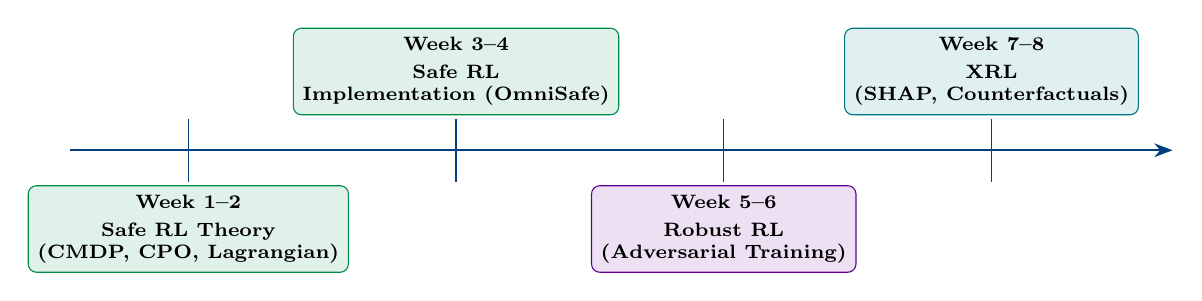
\begin{tikzpicture}[
    week/.style={draw=RLBlue,fill=RLBlue!10,rounded corners=3pt,
                 minimum width=3.0cm,minimum height=0.8cm,
                 font=\scriptsize\bfseries,align=center},
    topic/.style={draw=none,fill=none,font=\scriptsize,align=center}]
    \node[week,draw=SafeGreen,fill=SafeGreen!12]   at (0,-1)    {Week 1--2\\[2pt]Safe RL Theory\\(CMDP, CPO, Lagrangian)};
    \node[week,draw=SafeGreen,fill=SafeGreen!12]   at (3.4,1)  {Week 3--4\\[2pt]Safe RL\\Implementation (OmniSafe)};
    \node[week,draw=RobustPurple,fill=RobustPurple!12] at (6.8,-1) {Week 5--6\\[2pt]Robust RL\\(Adversarial Training)};
    \node[week,draw=ExplainTeal,fill=ExplainTeal!12] at (10.2,1) {Week 7--8\\[2pt]XRL\\(SHAP, Counterfactuals)};
    \draw[-Stealth,RLBlue,thick] (-1.5,0)--(12.5,0);
    \foreach \x in {0,3.4,6.8,10.2}
      \draw[RLBlue] (\x,0.4)--(\x,-0.4);
  \end{tikzpicture}
  \end{center}
  \vspace{0.3cm}
  \begin{columns}[T]
    \column{0.48\textwidth}
      \textbf{Weeks 1--2: Safe RL Theory}
      \begin{itemize}\scriptsize\setlength\itemsep{1pt}
        \item Read: Garcia \& Fernández survey; CPO paper
        \item Understand CMDPs and Lagrangian duality
        \item Run Safety-Gymnasium starter examples
      \end{itemize}
    \column{0.48\textwidth}
      \textbf{Weeks 7--8: XRL}
      \begin{itemize}\scriptsize\setlength\itemsep{1pt}
        \item Read: Milani et al. ACM survey on XRL
        \item Implement SHAP on a trained DQN
        \item Build Project 3: XRL Dashboard
      \end{itemize}
  \end{columns}
\end{frame}

%% ══════════════════════════════════════════════════
\section{Integrated RL Project (Phase 5 + 6)}
%% ══════════════════════════════════════════════════

\begin{frame}{Integrated Project: Safe \& Explainable RL Agent}
  \begin{columns}[T]
    \column{0.50\textwidth}
      \begin{block}{Project Overview}
        \textbf{Environment:} OpenAI Gymnasium \texttt{CartPole-v1} (extended with safety cost)\\[4pt]
        \textbf{Phase 5 contributions:}
        \begin{itemize}\small\setlength\itemsep{2pt}
          \item Offline RL: pre-train from logged CartPole data
          \item Meta-Learning: fast-adapt to perturbed pole lengths
        \end{itemize}
        \vspace{4pt}
        \textbf{Phase 6 contributions:}
        \begin{itemize}\small\setlength\itemsep{2pt}
          \item {\color{SafeGreen}Safety}: PPO-Lagrangian with angle cost
          \item {\color{RobustPurple}Robustness}: adversarial noise on observations
          \item {\color{ExplainTeal}Explainability}: SHAP + decision tree distillation
        \end{itemize}
      \end{block}
    \column{0.46\textwidth}
      \begin{tcolorbox}[colback=RLBlue!6,colframe=RLBlue,
                        title=\textbf{Jupyter Notebook Structure},
                        fonttitle=\small\bfseries]
        \scriptsize
        \begin{enumerate}\setlength\itemsep{3pt}
          \item \textbf{Setup}: Install deps, env creation
          \item \textbf{Baseline DQN}: train standard agent
          \item \textbf{Offline RL}: pre-training from replay
          \item \textbf{Safe RL}: add cost + PPO-Lagrangian
          \item \textbf{Robust RL}: adversarial attack + SA-DQN
          \item \textbf{XRL}: SHAP attribution plots
          \item \textbf{Policy Distillation}: decision tree
          \item \textbf{Dashboard}: compare all agents
        \end{enumerate}
      \end{tcolorbox}
      \vspace{4pt}
      \begin{center}
        \small\faGithub\ Full code available at:\\
        \href{https://github.com/abdullahzahid655}{\color{RLBlue}\texttt{github.com/abdullahzahid655}}
      \end{center}
  \end{columns}
\end{frame}

%% ══════════════════════════════════════════════════
\section{Summary \& Next Steps}
%% ══════════════════════════════════════════════════

\begin{frame}{Phase 6 Summary}
  \begin{columns}[T]
    \column{0.50\textwidth}
    \vspace{-11pt}
      \begin{block}{What We Covered}
        \begin{enumerate}\setlength\itemsep{3pt}\small
          \item \textbf{Safe RL}: CMDPs, Lagrangian methods, CPO, SafeDreamer, CBFs
          \item \textbf{Robust RL}: adversarial attacks, SA-MDP, RADIAL-RL, domain randomisation
          \item \textbf{XRL}: SHAP, saliency, counterfactuals, policy distillation, taxonomy
          \item \textbf{Synergies}: safe MARL, robust meta-RL, safe offline RL
          \item \textbf{Industry}: Waymo, Boston Dynamics, power grids, healthcare
        \end{enumerate}
      \end{block}
    \column{0.46\textwidth}
      \begin{exampleblock}{Key Insights}
        \begin{itemize}\setlength\itemsep{3pt}\small
          \item Safety $\neq$ Robustness $\neq$ Explainability — each addresses a different deployment risk
          \item All three are needed for real-world deployment
          \item Combining with Phase 5 paradigms unlocks the most powerful systems
          \item Active research area — new papers weekly
        \end{itemize}
      \end{exampleblock}
  \end{columns}
  \vspace{0.3cm}
  \begin{tcolorbox}[colback=RLOrange!8,colframe=RLOrange,
                    title=\textbf{Coming Next — Phase 7: Model-Based RL \& World Models},
                    fonttitle=\small\bfseries]
    \small
    Learning dynamics models, Dyna, Dreamer, MuZero, planning with uncertainty — the key to sample efficiency.
  \end{tcolorbox}
\end{frame}

\begin{frame}[plain]
  \begin{tikzpicture}[remember picture, overlay]
    \fill[RLBlue!95] (current page.south west) rectangle (current page.north east);
    \fill[RLOrange] ([yshift=-0.8pt]current page.north west)
                   rectangle ([yshift=-6pt]current page.north east);
  \end{tikzpicture}
  \begin{center}
    \vspace{0.8cm}
    {\color{white}\Huge\bfseries Thank You!}\\[12pt]
    {\color{white!80}\large Questions \& Discussion}\\[18pt]
    {\color{RLOrange}\rule{0.4\textwidth}{0.8pt}}\\[12pt]
    {\color{white}\normalsize Follow the RL Roadmap Series:}\\[6pt]
    {\color{white}\small
      \faLinkedin\ \href{https://linkedin.com/in/abdullahzahid655}
        {\color{RLOrange}linkedin.com/in/abdullahzahid655}
      \qquad
      \faGithub\ \href{https://github.com/abdullahzahid655}
        {\color{RLOrange}github.com/abdullahzahid655}
    }\\[16pt]
    {\color{white!60}\normalsize
      \textit{``An unsafe, brittle, or opaque AI is not truly intelligent — it is merely lucky.''}}
  \end{center}
\end{frame}

\begin{frame}[allowframebreaks]{References}
  \begin{thebibliography}{99}\small
    \bibitem{cpo2017}
      Achiam, J. et al. (2017). \textit{Constrained Policy Optimization.} ICML.
    \bibitem{saferl-survey}
      Wachi, A. et al. (2024). \textit{A Survey of Constraint Formulations in Safe RL.} arXiv:2402.02025.
    \bibitem{safedreamer2024}
      Huang, W. et al. (2024). \textit{SafeDreamer: Safe RL with World Models.} ICLR. arXiv:2307.07176.
    \bibitem{xrl-survey-acm-2023}
      Milani, S. et al. (2023). \textit{XRL: A Survey and Comparative Review.} ACM Comput. Surv.
    \bibitem{xrl-ml-2024}
      Bekkemoen, Y. (2024). \textit{XRL: Systematic Literature Review.} Machine Learning 113.
    \bibitem{sadqn2020}
      Zhang, H. et al. (2020). \textit{Robust DRL against Adversarial Perturbations.} NeurIPS 2020 (Spotlight).
    \bibitem{radial2021}
      Oikarinen, T. et al. (2021). \textit{RADIAL-RL.} NeurIPS 2021.
    \bibitem{robust-survey2024}
      Schott, L. et al. (2024). \textit{Robust DRL: Adversarial Attacks and Training Survey.} arXiv:2403.00420.
    \bibitem{fisor2024}
      Liu, Z. et al. (2024). \textit{FISOR: Feasibility-guided Safe Offline RL.} ICLR 2024.
    \bibitem{shap-xrl2024}
      Pakina, A. et al. (2024). \textit{AI Governance via XRL for Cyber Deception.} JISEM 2024.
    \bibitem{counterfactual-rl2024}
      Amitai, Y. et al. (2024). \textit{Explaining RL Agents via Counterfactual Action Outcomes.} AAAI 2024.
    \bibitem{arm-saferl2024}
      Adjei, P. et al. (2024). \textit{Safe RL for Arm Manipulation with CMDP.} Robotics, MDPI 13(4).
    \bibitem{beechey2023}
      Beechey, D. et al. (2023). \textit{Explaining RL with Shapley Values.} ICML 2023.
  \end{thebibliography}
\end{frame}

\end{document}